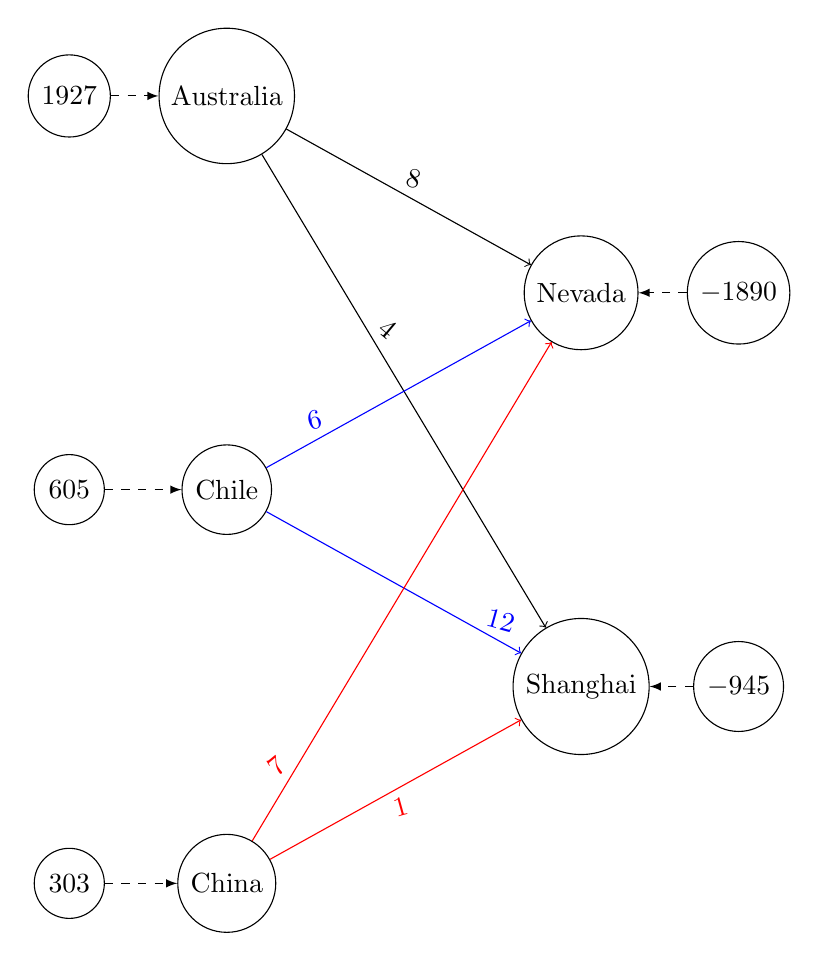
\begin{tikzpicture}[xscale=0.5]
  \def\x{1}
  \def\z{10}
  \def\y{2.5}

  \node[draw=black, circle] (AUS) at (\x, 0) {Australia};
  \node[draw=black, circle] (CHI) at (\x, -2 * \y) {Chile};
  \node[draw=black, circle] (CHINA) at (\x, -4 * \y) {China};

  \node[draw=black, circle] (Nevada) at (\z, -1 * \y) {Nevada};
  \node[draw=black, circle] (Shanghai) at (\z, -3 * \y) {Shanghai};

  \draw[->] (AUS) -- (Nevada) node [pos=0.5, above, sloped] {8};
  \draw[->] (AUS) -- (Shanghai) node [pos=0.4, above, sloped] {4};
  \draw[->] (CHI)[blue] -- (Nevada) node [pos=0.2, above, sloped] {6};
  \draw[->] (CHI)[blue] -- (Shanghai) node [pos=0.9, above, sloped] {12};
  \draw[->] (CHINA)[red] -- (Nevada) node [pos=0.12, above, sloped] {7};
  \draw[->] (CHINA)[red] -- (Shanghai) node [pos=0.5, below, sloped] {1};

  \draw node[circle, draw] (1) at (-3, 0 * \y) {$1927$};
  \draw node[circle, draw] (2) at (-3, -2 * \y) {$605$};
  \draw node[circle, draw] (3) at (-3, -4 * \y) {$303$};
  \draw node[circle, draw] (4) at (14, -1 * \y) {$-1890$};
  \draw node[circle, draw] (5) at (14, -3 * \y) {$-945$};

  \draw[dashed, -latex] (1)--(AUS);
  \draw[dashed, -latex] (2)--(CHI);
  \draw[dashed, -latex] (3)--(CHINA);
  \draw[dashed, -latex] (4)--(Nevada);
  \draw[dashed, -latex] (5)--(Shanghai);
\end{tikzpicture}
